\documentclass[10pt]{article}

\usepackage[margin=1in]{geometry}
\usepackage{times}
\usepackage{amsmath,amssymb,amsthm}
\usepackage{algorithm}
\usepackage{algorithmic}
\usepackage{enumitem}
\usepackage{graphicx}
\usepackage[hidelinks]{hyperref}
\usepackage[numbers]{natbib}
\usepackage{booktabs}
\usepackage{multirow}
\usepackage[table]{xcolor}
\usepackage{caption}
\usepackage{tikz}
\usetikzlibrary{shapes,arrows,positioning,calc}

\theoremstyle{definition}
\newtheorem{definition}{Definition}[section]

\title{Human--Agent Interaction for Dynamic Channel Assignment\\
       in Autonomous Drone Swarms}
\author{}
\date{}

\begin{document}
\maketitle

\begin{abstract}
We present a controlled laboratory platform for studying how human operators interact with
AI advisory agents when managing communication channels in a simulated drone swarm.  The
task is grounded in dynamic graph colouring: drones are graph nodes, proximity-based radio
links are edges, and the three available communication channels (Red, Green, Blue) are
colours.  Two drones on the same channel within radio range of each other experience
interference --- a colour clash in graph-theoretic terms.  Because the drones move
continuously, the interference graph changes in real time.  The key manipulation is
\emph{swarm complexity}, controlled by varying drone count and movement speed across
scenarios.  Operators manage channel assignments using one of five interaction modalities:
\emph{manual} individual reassignment (M1); \emph{batch suggestion} with human review
(M2); \emph{batch auto-assign} without review (M3); and two \emph{persistent-watch} modes
in which selected drones are continuously monitored by the agent --- either surfacing a
suggestion for human review (M4) or applying fixes autonomously (M5).  A second independent
variable, \emph{agent mode} (reactive vs.\ proactive), determines whether M4/M5 are
available.  The central question is how operators distribute effort across these modalities
as swarm complexity and agent proactivity increase, and whether this distribution reflects
appropriate calibration of trust to the agent's known imperfection.
\end{abstract}

%% ============================================================
\section{Introduction}
\label{sec:intro}
%% ============================================================

Autonomous drone swarms are increasingly deployed in scenarios --- search and rescue,
infrastructure inspection, distributed sensing --- that require persistent inter-drone
communication.  When drones operate on shared radio frequencies, proximity creates
interference: two drones within radio range of each other on the same frequency channel
cannot communicate reliably.  Assigning channels so that no two proximate drones share one
is a graph colouring problem, with drones as nodes and mutual radio range as
edges~\citep{mishra2005weighted}.

In static deployments this problem is solved offline.  In dynamic swarms, however, the
interference graph evolves as drones move, and valid channel assignments must be continuously
maintained.  Human-in-the-loop systems address this by letting a ground operator monitor the
swarm and issue channel reassignments.  But as swarm size and speed increase, the cognitive
demand of manual management grows and the case for AI assistance strengthens.

The question we study is not simply \emph{whether} AI assistance helps, but \emph{how
operators use it} and \emph{whether their reliance is well-calibrated}.  We provide
operators with an imperfect advisory agent --- one that produces valid, clash-free assignments
roughly 80\% of the time but occasionally makes random recommendations --- and observe how
they distribute usage across interaction modalities of increasing automation.

Under the \emph{reactive} agent mode, operators retain full initiative: they select drones
and request assistance on demand (M1--M3).  Under the \emph{proactive} (flexible) agent
mode, operators additionally designate individual drones as persistent monitors; the agent
then autonomously detects clashes within each monitored group and either surfaces a
suggestion (M4) or applies a fix directly (M5), without operator initiation.

Our contributions are:
\begin{enumerate}
  \item A formal model of the dynamic channel assignment task as online graph colouring,
        including a precise characterisation of geometrically infeasible configurations.
  \item An interface design with five interaction modalities spanning a spectrum from full
        human control to fully delegated automation.
  \item An imperfect advisory agent model for both on-demand and persistent clash monitoring.
  \item A $3 \times 2$ study design in which swarm complexity and agent mode are the
        independent variables and modality distribution is the primary dependent variable.
\end{enumerate}

%% ============================================================
\section{Formal Model}
\label{sec:model}
%% ============================================================

\subsection{Drones and Arena}

Let $\mathcal{D} = \{d_0, d_1, \ldots, d_{n-1}\}$ be a set of $n$ drones.  Each drone $d_i$
occupies position $\mathbf{p}_i(t) \in [0, W] \times [0, H]$ at time $t$.  Each drone is
assigned a communication channel $c_i(t) \in \mathcal{C} = \{\text{Red},\,\text{Green},\,\text{Blue}\}$,
or is in a transitional state $c_i(t) = \bot$ while a channel switch propagates.

\subsection{Proximity Graph and Interference}

At each instant $t$, the \emph{interference graph} $G(t) = (\mathcal{D},\, E(t))$ is defined by:
\begin{equation}
  (d_i, d_j) \in E(t) \iff \|\mathbf{p}_i(t) - \mathbf{p}_j(t)\| \leq d_{\mathrm{link}}
  \label{eq:edge}
\end{equation}
where $d_{\mathrm{link}}$ is the radio range radius (Section~\ref{sec:params}).
A pair $(d_i, d_j) \in E(t)$ is a \emph{clash} if both are on the same channel:
\begin{equation}
  \mathcal{K}(t) = \bigl\{(i,j) \in E(t) \mid c_i(t) = c_j(t) \neq \bot\bigr\}
  \label{eq:clash}
\end{equation}

\subsection{Infeasible Configurations}
\label{sec:infeasible}

Because only three channels are available, configurations in which more than three drones are
mutually within radio range --- a clique of size $\omega(G(t)) > 3$ --- cannot be properly
coloured.  In a bounded 2D arena, such cliques arise transiently as drones converge, are
geometrically possible, and cannot always be avoided by the operator.  These configurations
are an intentional feature of the task: they force the operator to \emph{minimise rather than
eliminate} clashes for a period, requiring prioritisation of which clashes to resolve first.

When a clique of size 4 is present, at least one clash pair must exist regardless of the
channel assignment.  The operator and advisory agent are both working in a locally infeasible
regime; the agent detects this condition and proposes a minimum-clash (rather than clash-free)
assignment.

\subsection{Performance Metric}

The primary performance measure is cumulative clash time over the trial duration $T$:
\begin{equation}
  T_{\mathrm{clash}} = \int_0^{T} \mathbf{1}\bigl[\mathcal{K}(t) \neq \emptyset\bigr]\, \mathrm{d}t
  \label{eq:metric}
\end{equation}
This penalises any period during which at least one clash exists, regardless of how many.
Complementary measures include the number and duration of individual clash episodes and the
number of channel switches issued (a proxy for operator workload).

\subsection{Channel Switching}

An operator action at time $t$ queues a switch for drone $d_i$ to channel $c'$, completed
after propagation delay $\tau$:
\[
  c_i(t + \tau) \leftarrow c'
\]
Only one pending switch per drone is permitted at a time.  During switching, $c_i = \bot$.
The delay $\tau$ is a key task parameter: it forces anticipatory action and makes the
interaction non-trivial (Section~\ref{sec:params}).

\subsection{Warning Zone}

A secondary threshold $d_{\mathrm{warn}} > d_{\mathrm{link}}$ defines an
\emph{approaching zone}.  Pairs within $d_{\mathrm{warn}}$ but not yet within $d_{\mathrm{link}}$
are visually flagged.  Because the maximum closing speed of two drones is
$v_{\max,\,\mathrm{close}} = 2 v_{\max}$, the warning zone affords advance notice of
approximately:
\[
  \Delta t_{\mathrm{warn}} \approx \frac{d_{\mathrm{warn}} - d_{\mathrm{link}}}{2\,v_{\max}}
\]
This is the window in which a switch initiated in Mode~M1 can complete before the link forms.

%% ============================================================
\section{Swarm Complexity}
\label{sec:complexity}
%% ============================================================

Complexity is the primary between-scenario variable.  It is jointly determined by:
\begin{itemize}
  \item \textbf{Drone count} $n$: more drones increase graph density and the rate of clash
        events.
  \item \textbf{Movement speed} $[v_{\min}, v_{\max}]$: faster drones produce more rapid
        topology changes, shorter warning windows, and more frequent transient
        cliques.
\end{itemize}

We define three named complexity levels, shown in Table~\ref{tab:complexity}.  Drone count
and speed range are co-varied so that each level represents a qualitatively distinct operating
regime.

\begin{table}[h]
\centering
\caption{Named complexity levels.  Speed range applies to each drone's randomly sampled
speed at each heading change.}
\label{tab:complexity}
\begin{tabular}{llcc}
\toprule
\textbf{Level} & \textbf{Label} & \textbf{Drones} ($n$) & \textbf{Speed (px/s)} \\
\midrule
Low    & \textsc{Easy}   &  8 &  6--10 \\
Medium & \textsc{Medium} & 12 &  7--15 \\
High   & \textsc{Hard}   & 16 & 10--20 \\
\bottomrule
\end{tabular}
\end{table}

At \textsc{Easy}, a skilled operator can likely manage the swarm manually with modest effort.
At \textsc{Hard}, the rate of new clash events should exceed what a human can handle by point-and-click alone, making batch operations and agent assistance valuable.  \textsc{Medium} is the transitional regime where we expect the most variation in individual operator strategy.

%% ============================================================
\section{Movement Model}
\label{sec:movement}
%% ============================================================

Each drone follows a \emph{bounded random walk}:

\paragraph{Heading updates.}
Drone $d_i$ selects a new heading at random intervals
$\Delta t_i \sim \mathrm{Uniform}(4, 9)$\,s.
At each update, the heading is perturbed by
$\delta \sim \mathrm{Uniform}(-\pi/3, +\pi/3)$
and speed is resampled from $\mathrm{Uniform}(v_{\min}, v_{\max})$.
Between updates, the drone gradually steers toward the committed heading at a maximum rate
of $\pi/2$\,rad/s, producing smooth curved trajectories rather than abrupt turns.

\paragraph{Boundary reflection.}
Drones reflect off arena walls with axis-appropriate velocity reversal.

\paragraph{Body separation.}
When two drone bodies overlap, they are pushed apart and the approaching component of relative
velocity is cancelled.  This prevents physical clustering while allowing their radio ranges
to overlap freely.

\paragraph{Reproducibility.}
All random draws come from a single seeded \texttt{random.Random} instance, so any scenario
is fully reproducible given its seed.

%% ============================================================
\section{Interaction Modalities}
\label{sec:modalities}
%% ============================================================

The operator may interact with the swarm using up to five modalities.  Modalities M1--M3 are
always available (\emph{reactive} mode).  Modalities M4--M5 are additionally available when
the agent mode is set to \emph{proactive} (Section~\ref{sec:flexible}).

\subsection{M1: Manual Individual Reassignment}

The operator clicks a single drone in the arena to select it.  A small popup appears above
the drone containing three channel buttons (Red, Green, Blue).  The current channel is
shown disabled; clicking another channel queues a $\tau$-second switch.  This modality offers
maximum operator control at the cost of throughput: reassigning $k$ drones requires $k$
separate click sequences.

\subsection{M2: Batch Suggestion with Review}

\paragraph{Selection.}
The operator selects a \emph{group} of drones by either (a) clicking and dragging to draw a
rectangular bounding box in the arena, capturing all drones within it, or (b)
\texttt{Ctrl}+clicking individual drones to add or remove them from the selection.

\paragraph{Requesting a suggestion.}
With one or more drones selected, the operator clicks ``Suggest'' in the control panel.  The
advisory agent (Section~\ref{sec:agent}) computes a proposed channel assignment for the
selected drones and returns it within one frame.

\paragraph{Review panel.}
The proposed assignment is shown in a \emph{suggestion panel}: a list of selected drones,
each with its current channel and the agent's proposed channel.  The operator may
(a) accept the proposal for each drone individually, (b) override the proposal for specific
drones by selecting a different channel, or (c) cancel the entire suggestion.  Clicking
``Apply'' queues a $\tau$-second switch for each drone whose proposed (or manually overridden)
channel differs from its current one.  If the operator manually reassigns a drone (M1) while
a suggestion is pending, the suggestion is immediately discarded.

\subsection{M3: Batch Auto-Assign}

Selection is performed identically to M2.  The operator then clicks ``Auto-assign'' instead
of ``Suggest''.  The advisory agent computes the same proposal as in M2, but it is applied
immediately without displaying the review panel.  Switches are queued for all selected
drones whose proposed channels differ from their current ones.

\paragraph{Design rationale.}
M3 maximises throughput and minimises operator effort, but fully delegates the channel
decision to the agent.  When the agent's proposal contains errors --- which it will
approximately 20\% of the time on any given drone --- M3 will apply those errors silently.
M2 allows the operator to catch and correct agent errors before they take effect, but at the
cost of a review step.  M1 bypasses the agent entirely.

The three modalities M1--M3 are always available simultaneously; the operator chooses freely
among them at any moment during the trial.

%% ============================================================
\section{Proactive (Flexible) Agent Mode}
\label{sec:flexible}
%% ============================================================

In \emph{proactive} agent mode, operators can designate individual drones as persistent
\emph{watch targets}.  Once designated, the advisory agent continuously monitors the
interference graph and acts autonomously when a clash involving any watched drone is detected,
without the operator needing to select drones or press a button.

\subsection{Designation}

The operator selects a group of drones (same mechanism as M2/M3) and then clicks one of two
new buttons in the control panel:
\begin{itemize}
  \item \textbf{Watch: Suggest} --- assigns the selected drones to M4 mode, displayed with
        an amber ring.
  \item \textbf{Watch: Auto} --- assigns the selected drones to M5 mode, displayed with a
        teal ring.
\end{itemize}
Clicking the same button a second time for already-watched drones removes their designation.
A drone can only be in one watch mode at a time; designating it to the other mode replaces
the previous assignment.

\subsection{M4: Persistent Watch with Suggestion}

Every 500\,ms the agent scans the interference graph.  If a clash is detected involving any
M4-watched drone, and no suggestion is currently pending, the agent:
\begin{enumerate}
  \item Identifies the connected component of watched drones containing the clash.
  \item Runs the batch suggestion algorithm (Algorithm~\ref{alg:agent}) on that component.
  \item Surfaces the result in the review panel, as in M2.
\end{enumerate}
The operator reviews and applies or cancels as normal.  To prevent re-triggering while a
switch is in progress, all drones in the accepted suggestion are placed on a cooldown of
$\tau + 0.5$\,s after the operator clicks ``Apply''.

\subsection{M5: Persistent Watch with Auto-Fix}

When a clash involving an M5-watched drone is detected, the agent applies the channel fix
immediately (as in M3) without operator intervention.  Only drones not currently on cooldown
and not already mid-switch are eligible for auto-fixing.  Each fixed drone receives the same
$\tau + 0.5$\,s cooldown.  All autonomous actions are recorded in an \emph{agent log} panel
displayed at the bottom of the control panel, timestamped and colour-coded (teal for M5).

\subsection{Design Rationale}

M4 and M5 shift the locus of initiative from the operator to the agent.  Under M4, the agent
\emph{monitors} and \emph{alerts}; human oversight is preserved.  Under M5, the agent acts
autonomously; the operator's role degrades to configuration and exception handling.  This
delegation spectrum --- from purely reactive (M1--M3, operator-initiated) to proactive
(M4, agent-alerted) to autonomous (M5, agent-acting) --- allows the study to examine how
willingness to delegate surveillance correlates with trust calibration and performance.

%% ============================================================
\section{Advisory Agent}
\label{sec:agent}
%% ============================================================

\subsection{Task}

Given a selected set of drones $S \subseteq \mathcal{D}$, the agent proposes a channel
assignment $\hat{c}: S \to \mathcal{C}$ that attempts to minimise clashes among all edges
incident to $S$ in $G(t)$, taking into account the current (fixed) channel assignments of
drones outside $S$.

\subsection{Algorithm}

The agent uses a greedy colouring with $\varepsilon$-random noise.

\begin{algorithm}
\caption{Imperfect Batch Channel Suggestion}
\label{alg:agent}
\begin{algorithmic}[1]
\REQUIRE Selected set $S$, current assignment $c$, edges $E(t)$, noise rate $\varepsilon$
\STATE Order $S$ by decreasing degree in $G(t)[S \cup \partial S]$
\FORALL{$d_i \in S$ in that order}
  \STATE $\mathrm{blocked} \gets \{c_j \mid (i,j) \in E(t),\ d_j \notin S \text{ or } d_j \text{ already assigned}\}$
  \STATE $\mathrm{free} \gets \mathcal{C} \setminus \mathrm{blocked}$
  \IF{$\mathrm{free} \neq \emptyset$}
    \STATE $c^*_i \gets \arg\min_{c \in \mathrm{free}} \text{(clash count with current partial assignment)}$
  \ELSE
    \STATE $c^*_i \gets \arg\min_{c \in \mathcal{C}} \text{(clash count)}$
    \COMMENT{infeasible subgraph: minimise rather than eliminate}
  \ENDIF
  \IF{$\mathrm{Uniform}(0,1) < \varepsilon$}
    \STATE $\hat{c}(d_i) \gets \mathrm{Uniform}(\mathcal{C})$
    \COMMENT{random noise replaces optimal}
  \ELSE
    \STATE $\hat{c}(d_i) \gets c^*_i$
  \ENDIF
\ENDFOR
\RETURN $\hat{c}$
\end{algorithmic}
\end{algorithm}

The noise parameter $\varepsilon = 0.20$ means each drone in the selected set has an
independent 20\% probability of receiving a randomly chosen channel rather than the
greedy-optimal one.  For a selection of $k$ drones, the probability that the entire
proposal is error-free is $(1-\varepsilon)^k$; for $k=5$ this is approximately 33\%.
This makes the agent useful but unreliable enough that uncritical M3/M5 usage imposes a
measurable performance cost.  The same algorithm is used for all five modalities; the
difference lies in who initiates it and how the result is handled.

\subsection{Infeasibility Detection}

Before returning the proposal, the agent checks whether the selected subgraph (plus its
fixed neighbours) contains a clique of size $> |\mathcal{C}| = 3$.  If so, it annotates
the proposal with an infeasibility flag and a count of unavoidable remaining clashes.  This
information is displayed in the M2 review panel and is logged regardless of which modality
triggered the suggestion.

%% ============================================================
\section{Interface Design}
\label{sec:interface}
%% ============================================================

\subsection{Display Layout}

The interface runs across two windows.  The \emph{arena window} occupies the operator's
primary display and shows the live drone simulation.  The \emph{control panel window} is
positioned on a secondary display (or side-by-side in single-monitor mode) and shows all
interaction controls, the suggestion panel, and --- in proactive mode --- the agent log.
Both windows are resizable; all radii and drone positions scale proportionally to maintain
topology-identical gameplay across display configurations.

\subsection{Arena}

Each drone is rendered as a filled circle coloured by its current channel (Red/Green/Blue),
dimmed during switching.  A semi-transparent radio-range halo of radius $d_{\mathrm{link}}/2$
surrounds each drone.  Overlapping halos indicate an active link; links whose endpoints share
a channel are drawn as red edges.  Approaching pairs within the warning zone are flagged with
amber rings.  In proactive mode, watch-target drones carry an additional coloured ring:
amber (thick) for M4 (Watch: Suggest) and teal (thick) for M5 (Watch: Auto).

\begin{figure}[t]
\centering
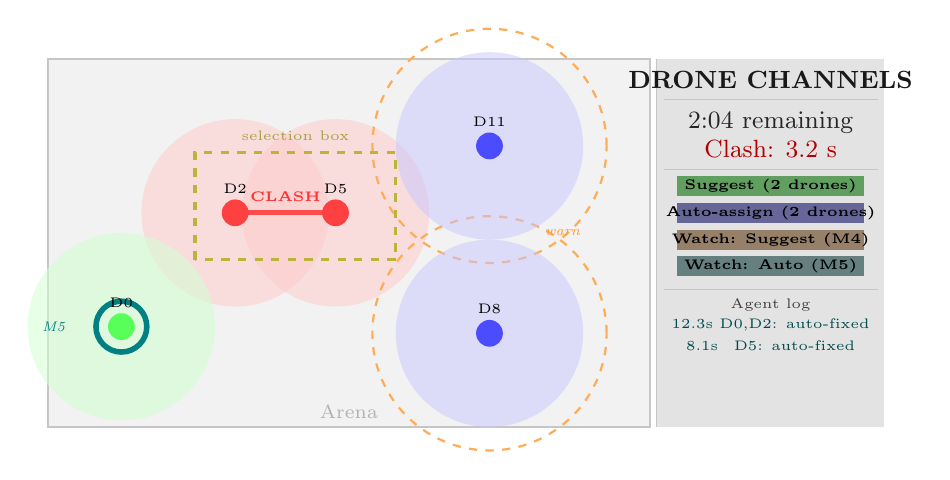
\begin{tikzpicture}[scale=0.85]
  % Arena
  \fill[gray!10] (0,0) rectangle (9,5.5);
  \draw[gray!45, thick] (0,0) rectangle (9,5.5);

  % --- Clashing pair (both Red) ---
  \fill[red!20, opacity=0.55] (2.8,3.2) circle (1.4);
  \fill[red!20, opacity=0.55] (4.3,3.2) circle (1.4);
  \draw[red!70, line width=1.8pt] (2.8,3.2) -- (4.3,3.2)
      node[midway, above, font=\tiny\bfseries, red!80] {CLASH};
  \fill[red!75] (2.8,3.2) circle (0.2);
  \fill[red!75] (4.3,3.2) circle (0.2);
  \node[font=\tiny] at (2.8,3.56) {D2};
  \node[font=\tiny] at (4.3,3.56) {D5};

  % --- Isolated drone (Green) with teal watch ring ---
  \fill[green!18, opacity=0.55] (1.1,1.5) circle (1.4);
  \fill[green!65] (1.1,1.5) circle (0.2);
  \draw[teal, line width=2pt] (1.1,1.5) circle (0.38);
  \node[font=\tiny] at (1.1,1.86) {D0};
  \node[font=\tiny, teal] at (0.1,1.5) {\textit{M5}};

  % --- Approaching pair (Blue, warning zone) ---
  \draw[orange!65, dashed, thick] (6.6,1.4) circle (1.75);
  \draw[orange!65, dashed, thick] (6.6,4.2) circle (1.75);
  \fill[blue!22, opacity=0.5] (6.6,1.4) circle (1.4);
  \fill[blue!22, opacity=0.5] (6.6,4.2) circle (1.4);
  \fill[blue!70] (6.6,1.4) circle (0.2);
  \fill[blue!70] (6.6,4.2) circle (0.2);
  \node[font=\tiny] at (6.6,1.76) {D8};
  \node[font=\tiny] at (6.6,4.56) {D11};
  \node[font=\tiny, orange!80] at (7.7,2.9) {\textit{warn}};

  % --- Bounding-box selection (dashed yellow rectangle) ---
  \draw[yellow!70!black, dashed, line width=1.2pt] (2.2,2.5) rectangle (5.2,4.1);
  \node[font=\tiny, yellow!60!black] at (3.7,4.35) {selection box};

  % Arena label
  \node[font=\scriptsize, gray!60] at (4.5,0.22) {Arena};

  % --- HUD Panel ---
  \fill[gray!22] (9.1,0) rectangle (12.5,5.5);
  \draw[gray!45] (9.1,0) -- (9.1,5.5);
  \node[font=\small\bfseries, gray!20!black] at (10.8,5.18) {DRONE CHANNELS};
  \draw[gray!45] (9.2,4.9) -- (12.4,4.9);
  \node[font=\small, gray!30!black] at (10.8,4.55) {2:04 remaining};
  \node[font=\small, red!70!black] at (10.8,4.15) {Clash: 3.2 s};
  \draw[gray!45] (9.2,3.85) -- (12.4,3.85);
  % Buttons (shown when group selected)
  \fill[green!25!gray] (9.4,3.45) rectangle (12.2,3.75);
  \node[font=\tiny\bfseries] at (10.8,3.60) {Suggest (2 drones)};
  \fill[blue!20!gray] (9.4,3.05) rectangle (12.2,3.35);
  \node[font=\tiny\bfseries] at (10.8,3.20) {Auto-assign (2 drones)};
  % Watch buttons (proactive mode only)
  \fill[orange!18!gray] (9.4,2.65) rectangle (12.2,2.95);
  \node[font=\tiny\bfseries] at (10.8,2.80) {Watch: Suggest (M4)};
  \fill[teal!20!gray] (9.4,2.25) rectangle (12.2,2.55);
  \node[font=\tiny\bfseries] at (10.8,2.40) {Watch: Auto (M5)};
  \draw[gray!45] (9.2,2.05) -- (12.4,2.05);
  % Agent log
  \node[font=\tiny, gray!50!black] at (10.8,1.82) {Agent log};
  \node[font=\tiny, teal!60!black] at (10.8,1.52) {12.3s  D0,D2: auto-fixed};
  \node[font=\tiny, teal!60!black] at (10.8,1.22) {8.1s\phantom{0}  D5: auto-fixed};
\end{tikzpicture}
\caption{Schematic interface layout.  Left: arena showing a clashing pair (red edge),
a drone with an M5 watch ring (teal), an approaching pair in the warning zone (amber dashed
rings), and a bounding-box selection in progress.  Right: the control panel, showing
context-sensitive M2/M3 buttons, M4/M5 watch-designation buttons (proactive mode only),
and the agent action log at the bottom.}
\label{fig:interface}
\end{figure}

\subsection{Selection and Group Actions}

When multiple drones are selected (Figure~\ref{fig:interface}), each is highlighted with a
cyan outline.  The HUD panel displays context-sensitive buttons: ``Suggest ($k$ drones)'',
``Auto-assign ($k$ drones)'', and, in proactive mode, ``Watch: Suggest'' and ``Watch: Auto''.
Single-drone selection shows the existing popup-style channel buttons (M1).

\subsection{Suggestion Panel (M2 / M4)}

On clicking ``Suggest'' (M2) or when M4 triggers autonomously, a panel shows:
\begin{itemize}
  \item Each selected drone's ID, current channel, and proposed channel (colour-coded).
  \item For each drone, per-channel override buttons to replace the proposed channel.
  \item An infeasibility warning if the subgraph cannot be 3-coloured.
  \item ``Apply'' and ``Cancel'' buttons.
\end{itemize}
Channels that would create a new clash are flagged in red.  Manual M1 reassignment of any
drone while a suggestion is pending immediately discards the suggestion.

\subsection{HUD Panel}

The control panel always shows:
\begin{itemize}
  \item \textbf{Timer}: time remaining, highlighted red below 20\,s.
  \item \textbf{Clash time}: cumulative seconds (the running score).
  \item \textbf{Context buttons}: Suggest / Auto-assign when a group is selected;
        Watch: Suggest / Watch: Auto additionally in proactive mode.
  \item \textbf{Instruction summary}: brief one-line reminders of each mode.
  \item \textbf{Agent log} (proactive mode): timestamped list of the eight most recent
        autonomous actions, colour-coded by mode (amber for M4, teal for M5).
\end{itemize}

%% ============================================================
\section{Data Logging}
\label{sec:logging}
%% ============================================================

All events are written as JSON objects to a timestamped JSONL file.
Each record contains a Unix wall-clock timestamp (\texttt{ts}) and the simulation time
(\texttt{elapsed}).  Table~\ref{tab:events} lists the event types.

\begin{table}[h]
\centering
\caption{Logged event types.  Mode column indicates which modality or system component
generates the event.}
\label{tab:events}
\begin{tabular}{llp{5.8cm}}
\toprule
\textbf{Event} & \textbf{Mode} & \textbf{Key payload fields} \\
\midrule
\texttt{game\_start}           & --    & seed, n\_drones, complexity, duration, agent\_mode \\
\texttt{switch\_requested}     & M1    & drone\_id, from, to, elapsed \\
\texttt{group\_selected}       & M2/M3 & drone\_ids, method (box/ctrl), elapsed \\
\texttt{suggestion\_requested} & M2    & drone\_ids, current\_channels, elapsed \\
\texttt{suggestion\_shown}     & M2/M4 & drone\_ids, proposed\_channels, infeasible \\
\texttt{suggestion\_modified}  & M2/M4 & drone\_id, proposed, overridden\_to \\
\texttt{suggestion\_applied}   & M2/M4 & final\_channels (proposed or overridden per drone) \\
\texttt{suggestion\_cancelled} & M2/M4 & elapsed \\
\texttt{auto\_assign\_applied} & M3/M5 & drone\_ids, proposed\_channels, infeasible, elapsed \\
\texttt{watch\_mode\_set}      & M4/M5 & drone\_ids, mode (suggest/auto), elapsed \\
\texttt{clash\_start}          & --    & elapsed, clashing\_pairs \\
\texttt{clash\_end}            & --    & elapsed, clash\_seconds\_so\_far \\
\texttt{game\_end}             & --    & elapsed, clash\_seconds, clash\_pct \\
\bottomrule
\end{tabular}
\end{table}

This event structure supports, among other analyses:
\begin{itemize}
  \item \textbf{Modality distribution}: the proportion of channel switches initiated via
        each of M1--M5 over the trial.
  \item \textbf{Agent override rate}: in M2/M4 sessions, how often the operator changed the
        agent's proposal for at least one drone.
  \item \textbf{Error detection}: comparison of \texttt{suggestion\_shown} and
        \texttt{suggestion\_applied} events reveals whether the operator caught agent errors.
  \item \textbf{Delegation depth}: the fraction of switches executed via autonomous M5
        relative to supervised M4, as a function of complexity and elapsed time.
  \item \textbf{Reaction latency}: time from \texttt{clash\_start} to the first relevant
        switch event.
\end{itemize}

%% ============================================================
\section{Study Design}
\label{sec:study}
%% ============================================================

\subsection{Design}

The study uses a $3 \times 2$ within-subjects design.  The two independent variables are:
\begin{description}[leftmargin=2em]
  \item[Swarm complexity] Three levels: \textsc{Easy}, \textsc{Medium}, \textsc{Hard}
        (Table~\ref{tab:complexity}).
  \item[Agent mode] Two levels: \emph{reactive} (M1--M3 only) and \emph{proactive}
        (M1--M5 available).
\end{description}
Trial ordering across the six conditions is counterbalanced.

\subsection{Procedure}

Each participant completes six 90-second trials, one per condition.  Participants are told
that the advisory agent is helpful but imperfect and that they should use their judgement
about when to rely on it.  They are not told the exact noise rate $\varepsilon$.

Prior to the main trials, a practice trial at \textsc{Easy} complexity familiarises
participants with all applicable modalities.  In proactive-mode practice, an on-screen
tutorial explains M4/M5 designation.

Post-trial questionnaires collect NASA-TLX workload ratings, a trust scale adapted
from~\citep{jian2000foundations}, and a free-text strategy report.

\subsection{Hypotheses}

\begin{description}[leftmargin=2em]
  \item[H1 \emph{(Performance vs.\ Complexity)}]
    $T_{\mathrm{clash}}$ will increase monotonically with complexity level.
  \item[H2 \emph{(Modality Shift with Complexity)}]
    The fraction of switches made via high-automation modes (M3, M5) will increase with
    complexity, as operators trade review thoroughness for throughput under cognitive load.
  \item[H3 \emph{(Over-reliance)}]
    The increase in M3/M5 usage at \textsc{Hard} complexity will be accompanied by a
    disproportionate increase in agent-induced errors, indicating over-reliance.
  \item[H4 \emph{(M2/M4 as a trust probe)}]
    The operator override rate in M2/M4 will correlate negatively with trial clash time,
    controlling for complexity.
  \item[H5 \emph{(Proactive mode and delegation)}]
    In proactive mode, operators who assign more drones to M5 (Watch: Auto) will show higher
    $T_{\mathrm{clash}}$ at \textsc{Hard} complexity than operators who prefer M4 (Watch:
    Suggest), due to undetected agent errors compounding under high topology change rates.
\end{description}

\subsection{Measures}

\paragraph{Primary.}
$T_{\mathrm{clash}}$: cumulative clash time (lower is better).

\paragraph{Behavioural.}
\begin{itemize}
  \item M1--M5 usage fractions (proportion of drone switches via each modality).
  \item M4/M5 designation rate: number of drones assigned as watch targets per trial.
  \item M2/M4 override rate: proportion of suggestions with at least one override.
  \item Selection size distribution in M2/M3.
  \item Reaction latency (clash onset to first switch action).
  \item Anticipatory rate: fraction of switches issued before a link forms (in warning zone).
\end{itemize}

\paragraph{Subjective.}
Post-trial NASA-TLX workload ratings; trust questionnaire adapted from~\citep{jian2000foundations};
free-text strategy report.

%% ============================================================
\section{Implementation}
\label{sec:impl}
\label{sec:params}
%% ============================================================

\begin{table}[h]
\centering
\caption{Source modules.}
\label{tab:components}
\begin{tabular}{lp{8.5cm}}
\toprule
\textbf{Module} & \textbf{Responsibility} \\
\midrule
\texttt{robot\_world.py}    & Physics: movement, collision separation, edge/clash detection,
                               switch queue, scaled instance radii. \\
\texttt{robot\_renderer.py} & All drawing: halos, edges, drone bodies, watch-mode rings,
                               selection highlights, suggestion panel, HUD, agent log,
                               overlays. \\
\texttt{robot\_game.py}     & Event loop: M1--M5 interaction, multi-select state,
                               suggestion request/apply/cancel, flexible-agent monitoring
                               tick, agent calls, logger calls. \\
\texttt{panel\_window.py}   & Separate OS window for the control panel using SDL2
                               hardware renderer; supports independent resizing. \\
\texttt{agents/channel\_agent.py} & Advisory agent: greedy colouring with $\varepsilon$-noise,
                               infeasibility detection. \\
\texttt{game\_logger.py}    & JSONL event logger. \\
\texttt{study\_runner.py}   & Study orchestrator: per-trial configuration (complexity,
                               agent mode, seed, duration), survey integration, output
                               directory management. \\
\texttt{launch\_menu.py}    & Standalone launcher GUI for single-session use outside the
                               formal study. \\
\texttt{tutorial.py}        & Scripted tutorial sequence shown before the first trial. \\
\texttt{surveys.py}         & Post-trial questionnaire windows (NASA-TLX, trust scale). \\
\bottomrule
\end{tabular}
\end{table}

The simulation runs at 60\,Hz; frame delta time is capped at 50\,ms.  All randomness (drone
movement and agent noise) is isolated in seeded \texttt{random.Random} instances for
reproducibility.  The agent runs synchronously in the game loop: for selections of up to
$\sim$20 drones the greedy algorithm completes in well under one frame.  All radii
($d_{\mathrm{link}}$, $d_{\mathrm{warn}}$, drone body radius) are computed at initialisation
as multiples of a reference arena width, so that topology is identical across display
resolutions.

\paragraph{Named complexity parameters.}

\begin{center}
\begin{tabular}{lccccc}
\toprule
\textbf{Level} & $n$ & $v_{\min}$ & $v_{\max}$ & $\Delta t_{\mathrm{turn}}$ & $\tau$ \\
\midrule
\textsc{Easy}   &  8 &  6 px/s & 10 px/s & 4--9 s & 3 s \\
\textsc{Medium} & 12 &  7 px/s & 15 px/s & 4--9 s & 3 s \\
\textsc{Hard}   & 16 & 10 px/s & 20 px/s & 4--9 s & 3 s \\
\bottomrule
\end{tabular}
\end{center}

%% ============================================================
\section{Conclusion}
\label{sec:conclusion}
%% ============================================================

We have described a platform for studying human--agent interaction in a real-time dynamic
channel assignment task.  The task is grounded in graph colouring, operationally motivated
by drone swarm spectrum management, and parameterised to span a range of operator cognitive
demands.  Five interaction modalities --- manual (M1), supervised batch suggestion (M2),
automated batch assignment (M3), persistent-watch suggestion (M4), and persistent-watch
auto-fix (M5) --- constitute a delegation spectrum that participants can navigate freely
during each trial.  A $3 \times 2$ design crossing swarm complexity with agent mode
(reactive vs.\ proactive) allows us to examine not only whether participants modulate their
use of high-automation modes in response to complexity, but also whether proactive agent
availability induces over-delegation, particularly when the agent's errors can compound
silently across multiple autonomous actions.

\bibliographystyle{plainnat}
\bibliography{refs}

\end{document}
